% 
% ======================================================================
\RequirePackage{desc-tex/styles/docswitch}
% \flag is set by the user, through the makefile:
%    make note
%    make apj
% etc.
\setjournal{\flag}

\documentclass[\docopts]{\docclass}

% You could also define the document class directly
%\documentclass[]{emulateapj}

% Custom commands from LSST DESC, see texmf/styles/lsstdesc_macros.sty
\usepackage{desc-tex/styles/lsstdesc_macros}

\usepackage{graphicx}
\graphicspath{{./}{./figures/}}
\bibliographystyle{desc-tex/bst/apj}

% Add your own macros here:



% 
% ======================================================================

\begin{document}

\title{The impact of LSST saturation on SN cosmology}

\maketitlepre

\begin{abstract}
We explore the impact of saturation on SN cosmology. In particular, we are interested in the effect of changing two equal timed snaps to a single snap in a visit. While a combination of bright supernovae (nearby), exceptionally good seeing in bluer bands can cause saturation for $30 s$ exposure all the way to $z = 0.05,$ the  combination of these uncommon factors is rare. When combined, it seems that the effect of saturation from $30~s$ exposures is small at redshifts $z \gtrsim 0.03$ 
\end{abstract}

% Keywords are ignored in the LSST DESC Note style:
\dockeys{latex: templates, papers: awesome}

\maketitlepost

% ----------------------------------------------------------------------
% 
\section{Introduction}
\label{sec:intro}
Survey strategy proposals frequently request that the default exposure time in LSST survey strategies
of $30~s$ per telescope visit or pointing be comprised of a single snap (or exposure), rather than the current two snaps of $15~s.$ While this proposal has advanatages, a disadvantage in doubling the exposure time is the collection of twice the number of photons during an exposure. For bright objects, such as nearby, near maximum supernovae, this could cross the full well depth of the CCD, so that pixels with counts higher than a theshold get saturated. This could happen for low redshift supernovae resulting in some of the light curve points being missing due to saturation. We look at the impact of this effect on SNIa cosmology.  

% ----------------------------------------------------------------------
\section{Methods}
\label{sec:methods}
To study the impact of saturation, our starting assumption is that the full well potential is 100,000. This is probably a good order of magnitude.

First, we calculate the number of photons collected in a single pixel from the sky as well as from a point source. This is shown in Figure.~\ref{fig:collected_photons}
\begin{itemize}
        \item We can calculate the number of photons collected (gain=1) from the magnitude in a band. This has been checked with using the lsst sims software. 
        \item This will be spread across a number of pixels. We use the approximation of a single Gaussian profile to model the PSF. The FWHM for this is known in terms of the standard deviation. We use this to calculate the density of photons at the brightest pixel, and multiply by the area to get the number of photons collected in the brightest pixel. 
        \item Given a sky brightness in mag/arc-sec, it is straightforward to calculate the number of photons from the sky collected. 
    \end{itemize}

Note this ignores other sources of photons such as a host galaxy. 

Second, we look directly at the effect on light curves of supernova Type Ia.


Finally, we take the results from an SNAANA simulation based on the \verb minion_1016  opsim output. This includes contributions such as a host galaxy as well.
\section{Results}
\label{sec:results}
\begin{figure}
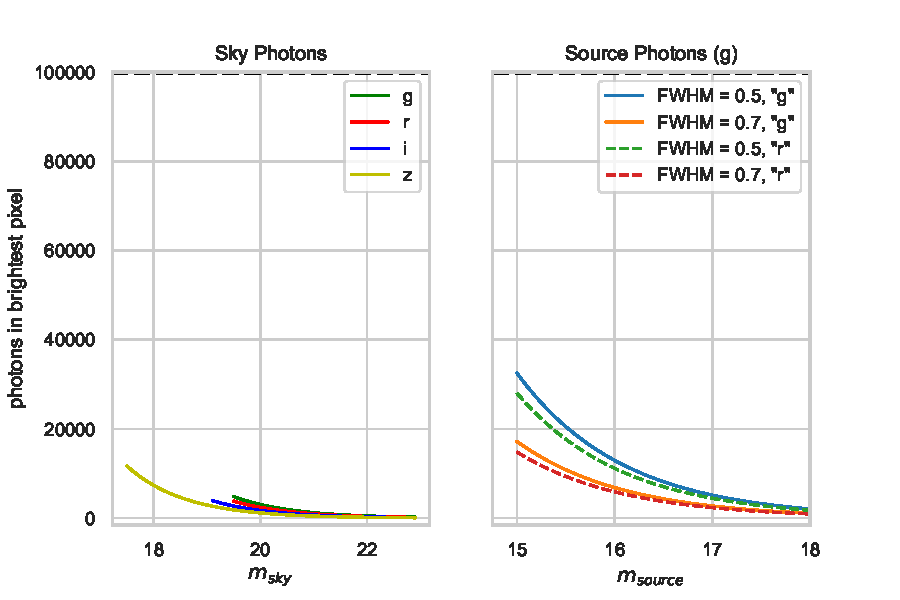
\includegraphics[width=0.9\columnwidth]{collected_photons}
\caption{Left: The number of sky photons per LSST pixel as a function of the sky brightness in units of $\mathrm{mag/arc-sec^2}$ in different bands of LSST. The ranges of $m_{sky}$ in different bands cover the range in OpSim (kraken\_2026 ). Right: The number of source photons in the brightest pixel for a source as a function of the source brightness in magnitude, for LSST bands g and r for minimum and median FWHM of 0.7\label{fig:collected_photons}}
\end{figure}
Figure~\ref{fig:collected_photons} shows that the number of sky photons collected in each pixel of the CCD is small compared to the assumed full well potential of $100000$ shown in a dashed horizontal line. This is high only for $z$ because there are observations in $z$ and $y$ when the sky is very bright. However, at the same sky brightness the redder bands contain far less photons. On the right panel,  figure shows that photon counts in the brightest pixel as a function of source brightness in different bands, as well as the seeing. While even for the brightest sky in $z$ the sky photons only gave about 20000 per pixel, we see that the a source even dimmer than 17 mags can saturate the brightest pixel at the best seeing conditions of the full width half maxima (FWHM) $\sim 0.5.$ This is the minimum of the seeing in $g$ band and the seeing rises sharply to median values of $\sim~0.7.$ Hence, most $g$ band obervations that lead to problems will probably be rare needing the combination of a rare seeing and sampling SN in a small volume near maxima.

In Figure.~\ref{fig:hubble},
\begin{figure}
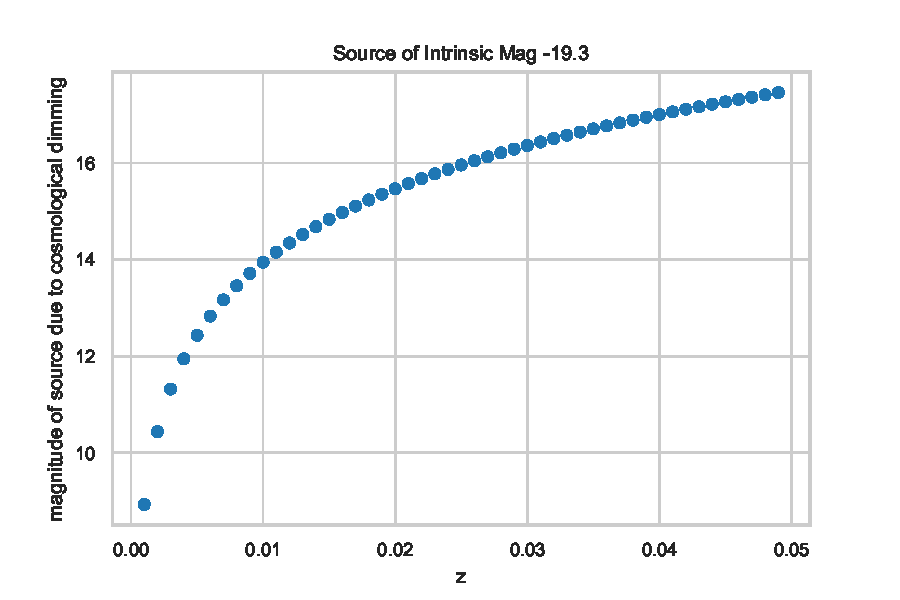
\includegraphics[width=0.9\columnwidth]{HubbleDiag}
\caption{The magnitude of a source with intrinsic magnitude of -19.3 mags\label{fig:hubble}}
\end{figure}
we look at the magnitudes of a source of absolute magnitude -19.3 including only the effect of cosmological dimming.


In Figure.~\ref{fig:standard_lc}, we look at the light curves of standard SNIa at a fixed absolute magnitude at different redshifts and seeing conditions. The number of photons in the brightest pixels is calculated. We can see that at lower redshifts, SNIa observed with very good seeing have observations clipped off due to saturation. However, these require the rare good seeing as well as nearby supernovae. This seems unlikelier at redshifts of $0.04, 0.05,$ though there are brighter SNIa than the average ones we chose to look at.

\begin{figure}
    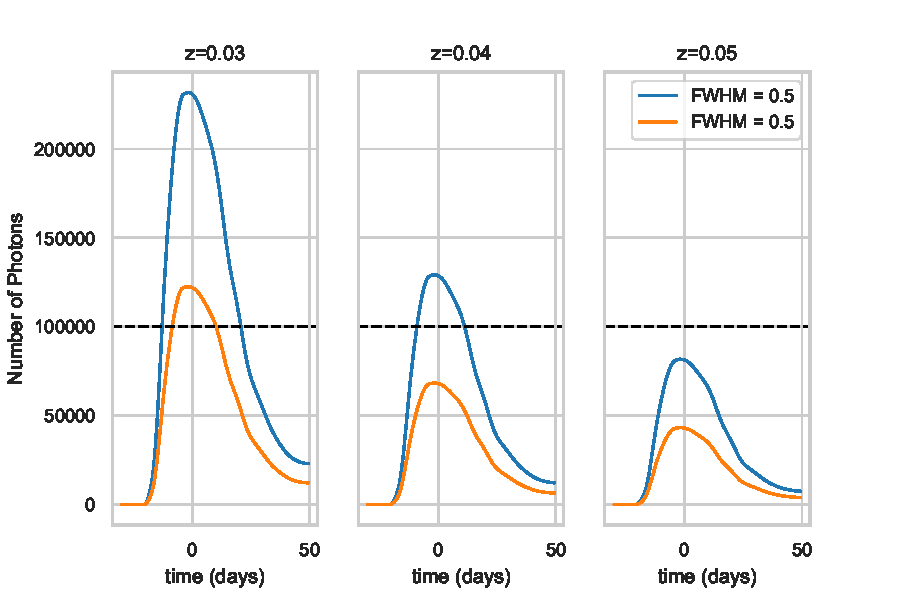
\includegraphics[width=0.9\columnwidth]{standard_lc}
    \caption{The number of photons for a SN with peak Absolute Magnitude $M_B = -19.3$ in the Bessell B band, at three different redshifts $0.03,~0.04,~0.05$ at FWHM of $0.5, 0.7$ with a dashed black horizontal line
       showing where the observations will be clipped off during saturation \label{fig:standard_lc}}
   \end{figure}
\begin{figure}
    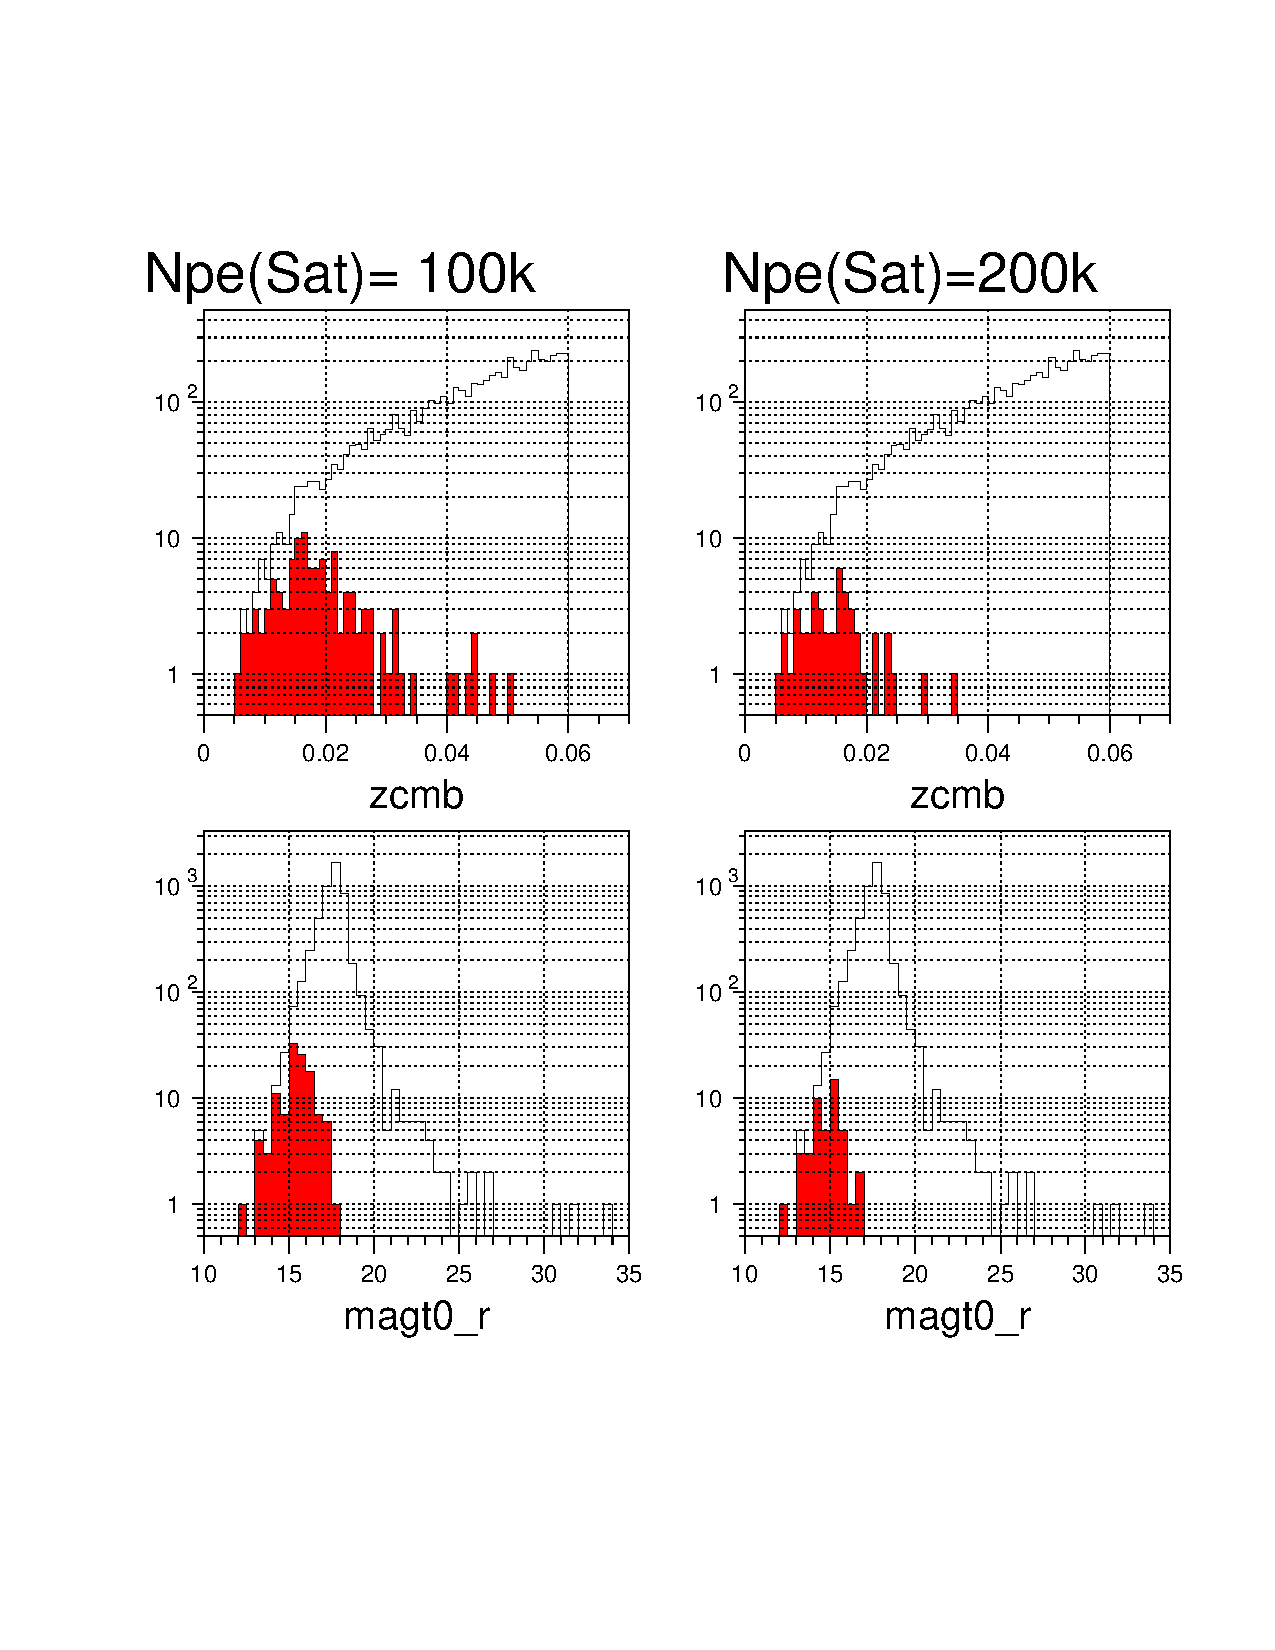
\includegraphics[width=0.4\columnwidth]{nobs_saturate_gt0}
    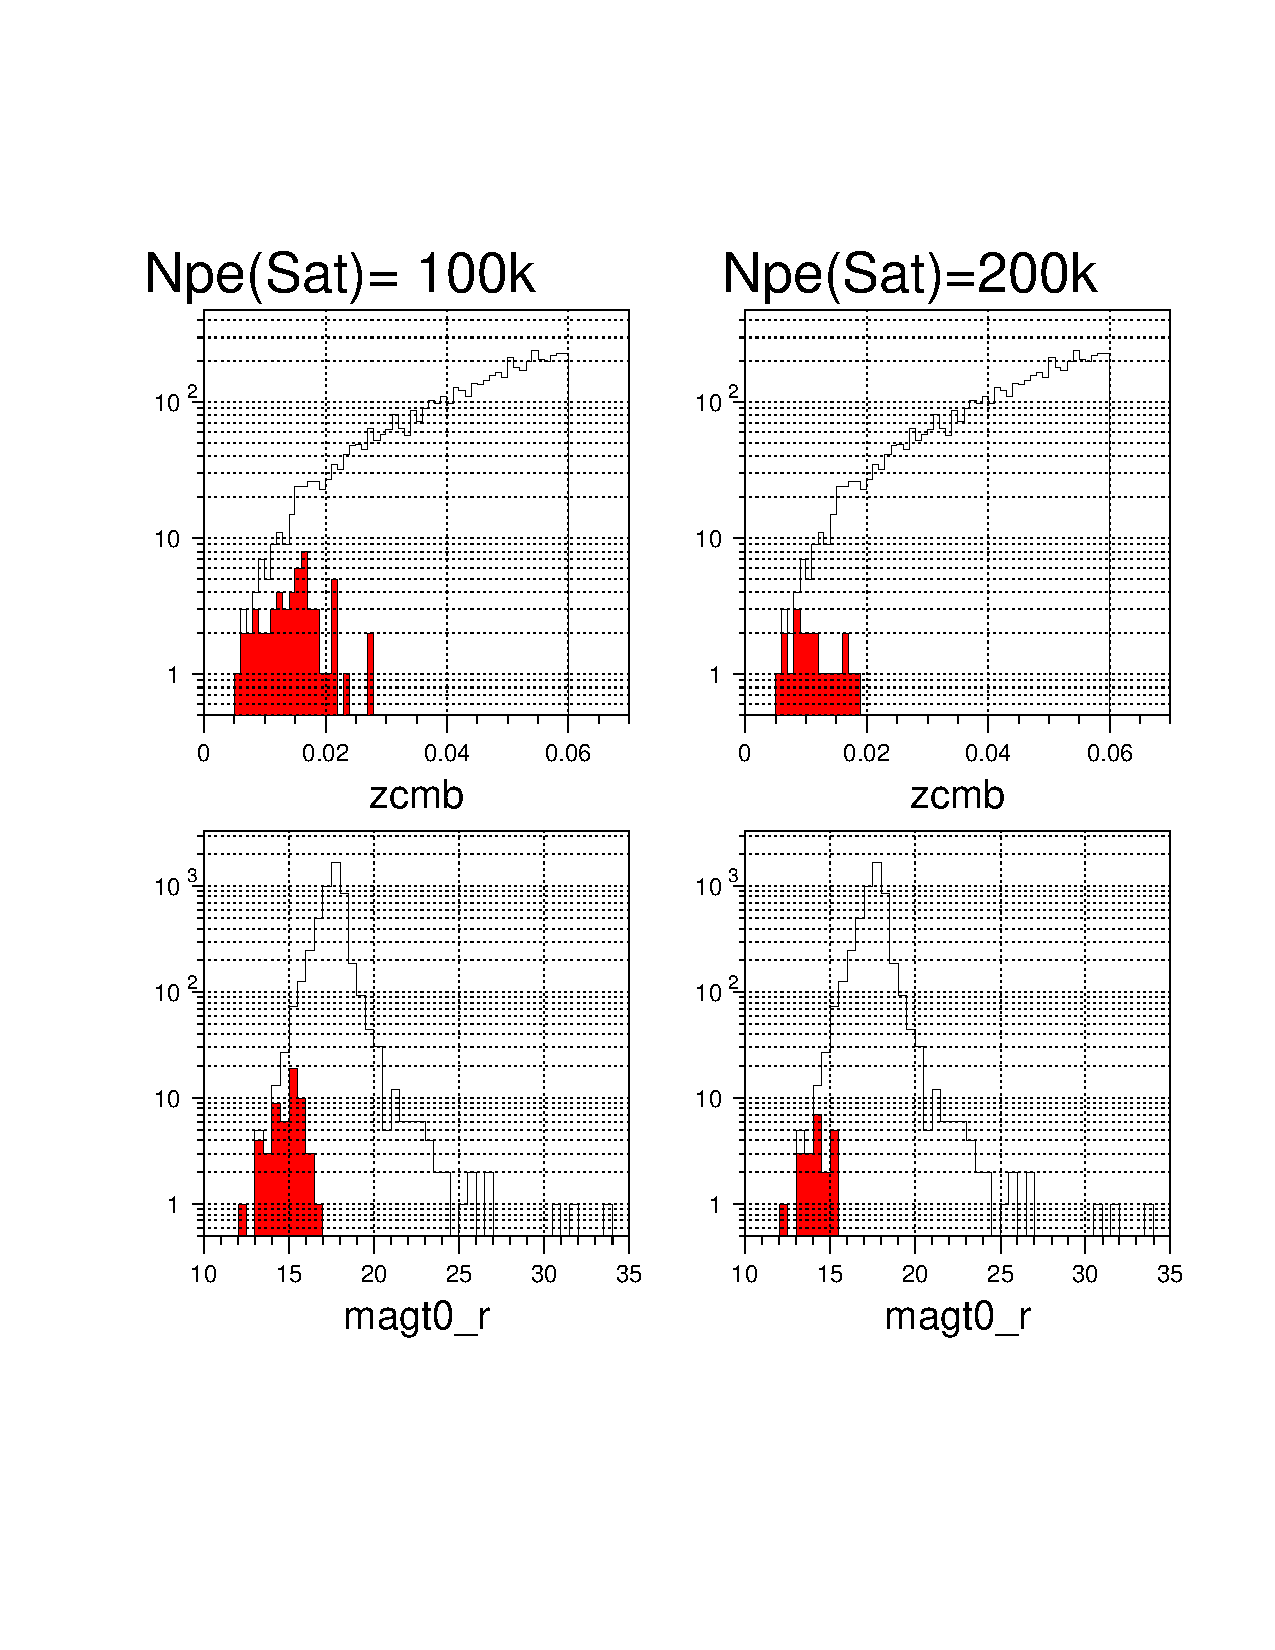
\includegraphics[width=0.4\columnwidth]{nobs_saturate_gt1}
    \caption{\textbf{Left:}~Histogram of SNIa (black) in an SNANA simulation based on minion\_1016, along with a histogram of SNIa (filled red) where at least one epoch was saturated as a function of magnitude at peak (lower) and redshift (upper) for 2 snaps (left column) and 1 snap (right column). \textbf{Right} Same but the filled red histogram is of SN with more than one epoch saturated. \label{fig:saturation_hist}}
\end{figure}

In Figure~\ref{fig:saturation_hist}, we include further possible contributions to the photon count. Secondly, we use a population of SNIa with the realistic distributions. These are then sampled using an opsim output. 
The result shows that while good conditions might prevent SNIa at low redshifts being observed, the fractin of cases where this happens is small.
\section{Discussion}
\label{sec:discussion}
Elsewhere, we have heard of a magnitude of 17 being a good estimate for when saturation kicks in. With a different reasonable assumption, we seem to be getting results in similar ballparks as expected.

% ----------------------------------------------------------------------

\section{Conclusions}
\label{sec:conclusions}

Saturation, even with a single 30 sec snap per visit likely does to have a problem till around z of 0.02-0.03. SNIa at redshifts greater than 0.03 seem largely unaffected by saturation. However, while highly uncommon, individual observations of SNIa might end up saturated upto redshifts close to 0.05. 

% ----------------------------------------------------------------------

\subsection*{Acknowledgments}

%Author contributions are listed below. \\
P.~Marshall: Initiated and led project, designed templates, tested system. \\
 % Standard papers only: author contribution statements. For examples, see http://blogs.nature.com/nautilus/2007/11/post_12.html
% Standard papers only: A.B.C. acknowledges support from grant 1234 from ...

The DESC acknowledges ongoing support from the Institut National de Physique Nucl\'eaire et de Physique des Particules in France; the Science \& Technology Facilities Council in the United Kingdom; and the Department of Energy, the National Science Foundation, and the LSST Corporation in the United States.  DESC uses resources of the IN2P3 Computing Center (CC-IN2P3--Lyon/Villeurbanne - France) funded by the Centre National de la Recherche Scientifique; the National Energy Research Scientific Computing Center, a DOE Office of Science User Facility supported by the Office of Science of the U.S.\ Department of Energy under Contract No.\ DE-AC02-05CH11231; STFC DiRAC HPC Facilities, funded by UK BIS National E-infrastructure capital grants; and the UK particle physics grid, supported by the GridPP Collaboration.  This work was performed in part under DOE Contract DE-AC02-76SF00515.
 % also available: key standard_short

\bibliography{main,desc-tex/bib/lsstdesc}

\end{document}
% ======================================================================
% 
